\documentclass[a4paper, titlepage]{article}
\usepackage[round, sort, numbers]{natbib}
\usepackage[utf8]{inputenc}
\usepackage{amsfonts, amsmath, amssymb, amsthm}
\usepackage{color}
\usepackage{listings}
\usepackage{marvosym}
\usepackage{mathtools}
\usepackage{paralist}
\usepackage{parskip}
\usepackage{subfig}
\usepackage{tikz}
\usepackage{titlesec}

\numberwithin{figure}{section}
\numberwithin{table}{section}

\usetikzlibrary{arrows, automata, backgrounds, petri, positioning}
\tikzstyle{place}=[circle, draw=blue!50, fill=blue!20, thick]
\tikzstyle{transition}=[rectangle, draw=black!50, fill=black!20, thick]

% define new commands for sets and tuple
\newcommand{\setof}[1]{\ensuremath{\left \{ #1 \right \}}}
\newcommand{\tuple}[1]{\ensuremath{\left \langle #1 \right \rangle }}
\newcommand{\card}[1]{\ensuremath{\left \vert #1 \right \vert }}

\makeatletter
\newcommand\objective[1]{\def\@objective{#1}}
\newcommand{\makecustomtitle}{%
	\begin{center}
		\huge\@title \\
		[1ex]\small Aurélien Coet, Dimitri Racordon
	\end{center}
	\@objective
}
\makeatother

\begin{document}

  \title{Outils formels de Modélisation \\ 3\textsuperscript{ème} séance d'exercices}
  \author{Aurélien Coet, Dimitri Racordon}
	\objective{
		Dans cette séance d'exercices, nous allons étudier et manipuler le comportement de réseaux de Petri en utlisant la simulation.
	}

	\makecustomtitle

  \section{Simulations [\Keyboard] ($\bigstar\bigstar$)}
    Représentez le réseau de Petri de la figure \ref{fig:bezout} en F\#,
    puis répondez aux questions suivantes:

    \begin{enumerate}
			\item La transition $t_2$ est-elle tirable?
			\item Donnez un marquage possible du réseau après 100 tirs de transitions.
		\end{enumerate}

    \begin{figure}[ht]
      \centering
        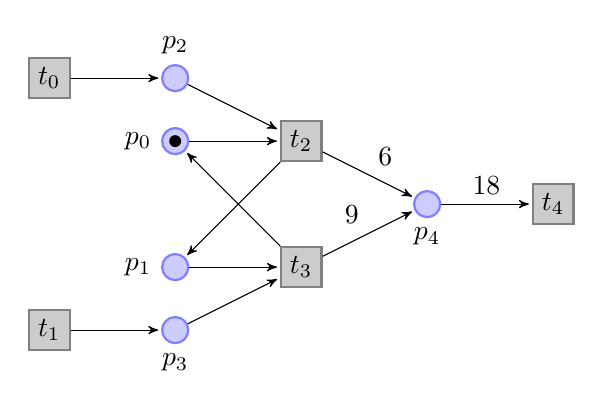
\begin{tikzpicture}[node distance=16mm, >=stealth', bend angle=45, auto]
          \node[place] (p4) [label=below:$p_4$] {};
          \node[place,tokens=1] (p0) [left of=p4,xshift=-16mm,yshift=8mm,label=left:$p_0$] {};
          \node[place] (p1) [left of=p4,xshift=-16mm,yshift=-8mm,label=left:$p_1$] {};
          \node[place] (p2) [above of=p0,yshift=-8mm,label=above:$p_2$] {};
          \node[place] (p3) [below of=p1,yshift=8mm,label=below:$p_3$] {};

          \node [transition] (t0) [left of=p2] {$t_0$}
                edge [post] (p2);
          \node [transition] (t1) [left of=p3] {$t_1$}
                edge [post] (p3);
          \node [transition] (t2) [right of=p0] {$t_2$}
                edge [pre] (p0)
                edge [pre] (p2)
                edge [post] node {6} (p4)
                edge [post] (p1);
          \node [transition] (t3) [right of=p1] {$t_3$}
                edge [pre] (p1)
                edge [pre] (p3)
                edge [post] node {9} (p4)
                edge [post] (p0);
          \node [transition] (t4) [right of=p4] {$t_4$}
                edge [pre] node[swap] {18} (p4);
        \end{tikzpicture}
      \caption{Réseau exposant des propriétés algébriques intéressantes}
      \label{fig:bezout}
    \end{figure}

  \section{Complémentaire mon cher [\Keyboard] ($\bigstar\bigstar$)}
		En cours, nous avons vu qu'il pouvait parfois être désirable d'ajouter une place
    qui limite le nombre de tokens pouvant être produits dans une autre place.
    On appelle généralement ces ajouts des \emph{places complémentaires}.

		Modifiez le réseau de Petri de la figure \ref{fig:bezout} pour y limiter le nombre de jetons dans chaque place à 36, \emph{sans autrement modifier le comportement du réseau}.

		Ecrivez ensuite la définition formelle d'une place complémentaire.
    Votre définition doit être de la forme suivantes:
    \emph{Soit $N$ un réseau de Petri tel que ... $p'\in P$ est dite complémentaire à $p \in P$ si et seulement si ...}

\end{document}
